\documentclass{optica-article}

%% Select the journal you're submitting to
%% oe, boe, ome, optcon, opticajournal
\journal{opticajournal}
% Key:
% Express journals must have the correct journal selected:
% {oe} Optics Express
% {boe} Biomedical Optics Express
% {ome} Optical Material Express
% {optcon} Optics Continuum
% Other Optica journals may use:
% {opticajournal} Applied Optics, Advances in Optics and Photonics, Journal of the Optical Society of America A/B, Optics Letters, Optica, Photonics Research

% Uncomment if submitting to Photonics Research.
% ONLY APPLICABLE FOR \journal{opticajournal}
% \setprjcopyright

% Set the article type
\articletype{Research Article}
% Note that article type is not required for Express journals (OE, BOE, OME and OPTCON)

\usepackage{lineno}
% \linenumbers

% ------------------------------------------------------------ Imported Packages
% \usepackage{graphicx}
% \usepackage{amsmath}
% \usepackage{amssymb}
% \usepackage{float}
% \usepackage{commath}
\usepackage{siunitx}
\usepackage{physics}
% \usepackage{subfigure}
\usepackage{hyperref}
% \usepackage{multicol}
\usepackage{subcaption}
\usepackage{epsfig}
\usepackage{xcolor}
\usepackage{cancel}

\AtBeginDocument{\RenewCommandCopy\qty\SI}

% LaTeX Functions
\newcommand{\dft}[2]{\frac{d^{#2}#1}{dt^{#2}}}
\DeclareMathOperator{\sinc}{sinc}
\DeclareMathOperator{\e}{e}
\DeclareMathOperator{\der}{d\hspace{-0.2em}}
\DeclareMathOperator{\proj}{proj}
\DeclareMathOperator{\sign}{sign}
\newcommand{\bX}[0]{\mathbf{X}}
\newcommand{\bv}[1]{\mathbf{#1}} 
\newcommand{\parallelsum}{\mathbin{\!/\mkern-5mu/\!}}
\newcommand{\vecc}[1]{\mathbf{#1}}

\begin{document}

\title{Maxwell's Equations in Anisotropic Materials: Half-Waveplates, 
Quarter-Waveplates, and Uniaxial Media}

\author{Kevin Lindstrom\authormark{1,*}}

\address{\authormark{1} Graduate Student, Department of Electrical and Computer
  Engineering, University of Connecticut, 371 Fairfield Way,
  Storrs, CT 06269-4157, USA.\\}

\email{\authormark{*}kevin.lindstrom@uconn.edu} %% email address is required; see note 
% below about the corresponding author designation

% \homepage{http:...} %% author's URL, if desired

%%%%%%%%%%%%%%%%%%% abstract %%%%%%%%%%%%%%%%
%% [use \begin{abstract*}...\end{abstract*} if exempt from copyright]

\begin{abstract}
  This paper discusses electromagnetic in uniaxial media and focuses on the 
  specific case of designing a waveplate. Waveplates are useful optical devices
  that change the polarization of an incident electromagnetic wave and are 
  used in many applications from research to photography. This report covers
  the necessary theoretical background that describes electromagnetic fields 
  in anisotropic materials, and derives series solutions for the output fields
  of a simple half-waveplate and quarter-waveplate. These analytical solutions
  were then used to design these waveplates using a quartz crystal for 590 nm 
  normally incident light. The performance of the designed waveplates was
  evaluated, and oblique incidence was discussed. Design challenges surrounding
  waveplate design were mentioned as well.
\end{abstract}

%%%%%%%%%%%%%%%%%%%%%%%%%%  body  %%%%%%%%%%%%%%%%%%%%%%%%%%
\tableofcontents

% ------------------------------------------------------------------------------
% Introduction
% ------------------------------------------------------------------------------
\section{Introduction}
Describing electromagnetic waves in anisotropic material is of practical
interest for describing designing many optical devices that are useful in 
research as well as the wider economy. This report will investigate a Maxwell's 
Equation based approach to modelling light in an anisotropic material and will
design a simple quartz half-waveplate (HWP) and quarter-waveplate (QWP) with 
this approach. Anisotropic materials are materials that have directional 
dependence to their constitutive parameters. Our discussion will primarily
focus on plane wave incidence on a birefringent material that has a ``fast'' 
and ``slow'' optical axis.
This nomenclature will be explained later on in the report.
We will start with the theoretical background that introduces the math necessary
to perform the design and analysis. It will be shown that for uniaxial
anisotropic media that the $\bv{\hat{x}}$,  $\bv{\hat{y}}$, and $\bv{\hat{z}}$ 
components of the wave equation remain uncoupled, and that this allows fields in 
$\bv{\hat{x}}$ and $\bv{\hat{y}}$ to propagate in $\bv{\hat{z}}$ independent 
of each other.

We will now have a brief aside about notation. In this report, most vectors will
be denoted by a bold variable, for example the electric field phasor 
$\bv{E}(x,y,z)$ and the unit vector $\bv{\hat{x}}$. Time varying fields, 
however, will be denoted by a script with a vector mark 
$\vec{\mathscr{E}}(x,y,z; t)$. Furthermore, matrices will be denoted by a
simple bar over the variable, like the dielectric matrix $\bar{\epsilon}$. 
Additional notation will be explained when necessary.


% ------------------------------------------------------------------------------
% Theory
% ------------------------------------------------------------------------------
\section{Theory}
The theory will be introduced from the most general to 
the specific such that the assumptions necessary for the waveplate design are
well substantiated, and the reader will be able to grasp more complex anisotropic
materials that will be lightly discussed later in the report. We begin our 
discussion with the displacement field $\vec{\mathscr{D}}(x,y,z; t)$.

% ------------------------------------------------------- The Displacement Field
\subsection{The Displacement Field}
As is discussed in \textit{Advanced Engineering Electromagnetics} time varying
fields can be analyzed in the phasor domain if they are time harmonic, and the
relationship between the time domain and phasor domain is as follows 
(shown in Cartesian coordinates for clarity)
\begin{equation}
\vec{\mathscr{D}}(x,y,z; t) = 
\mathfrak{Re}\left\{ e^{j\omega t}\bv{D}(x,y,z)\right\}
\end{equation}
where $\omega$ is the angular frequency of the time harmonic field 
\cite{Balanis-2012}. The displacement field $\vec{\mathscr{D}}(x,y,z; t)$ is 
a useful tool for analyzing the electric field in media and has units of
$\si{C\cdot m^{-2}}$. It
has the following
relationship to the electric field $\vec{\mathscr{E}}(x,y,z; t)$ for isotropic
media (media without directional dependent constitutive parameters)
\begin{equation}\label{eq:D_deff}
  \vec{\mathscr{D}}(x,y,z; t) = \epsilon_0 \vec{\mathscr{E}}(x,y,z; t) + 
  \vec{\mathscr{P}}(x,y,z; t) 
  = \epsilon \vec{\mathscr{E}}(x,y,z; t)
\end{equation}
where $\vec{\mathscr{P}}(x,y,z; t)$ is the polarization of the material---not to
be confused with the polarization of an electromagnetic (EM) wave. The above
relationship holds true in the phasor domain as well
\begin{equation}\label{eq:D_deff_ph}
  \bv{D}(x,y,z) = \epsilon_0 \bv{E}(x,y,z) + \bv{P}(x,y,z)
  = \epsilon \bv{E}(x,y,z)
\end{equation}
where in both Equation \eqref{eq:D_deff} and \eqref{eq:D_deff_ph} the material's
permittivity $\epsilon$ can be related to its relative permittivity $\epsilon_r$
\cite{griffithsEM}
\begin{equation}
\epsilon = \epsilon_0\epsilon_r
\end{equation}
At an interface from material 1 to 2, the parallel and perpendicular boundary 
conditions (BC) for the 
displacement field are
\begin{equation}\label{eq:D_BC}
  (\bv{D}_2 - \bv{D}_1)\cdot \bv{\hat{n}}_{12} = \sigma_f
\quad\text{and}\quad
  (\bv{D}_2 - \bv{D}_1) \times \bv{\hat{n}}_{12} =
 (\bv{P}_2 - \bv{P}_1) \times \bv{\hat{n}}_{12}
\end{equation}
respectively, where $\sigma_f$ is the free (unbounded) surface charge density at
the interface, and $\bv{\hat{n}}_{12}$
is the normal vector of the interface from medium 1 to medium 2 
\cite{griffithsEM}. These 
relationships are the same as saying that the tangential components of the 
electric field must be continuous at a dielectric-dielectric interface.
Now that we have introduced the displacement field, we now discuss the 
displacement field in anisotropic media.

% ---------------------------------------- Anisotropy and The Displacement Field
\subsection{Anisotropy and The Displacement Field}
Anisotropic materials are materials that are directional dependent, and for 
our discussion we will consider the case of directional dependence of the 
material's permittivity. Many materials in nature have this dependence as
their crystalline structure creates many small dipole moments that affect the
material's polarization. In the most broad sense, an anisotropic material's
relative permittivity can be written as a rank 2 tensor (a matrix) 
\cite{Balanis-2012,CWA_S,Wav_anis}
\begin{equation}\label{eq:eps_ten}
  \bar{\epsilon}_r = \begin{bmatrix}
      \epsilon_{xx} & \epsilon_{xy} & \epsilon_{xz}\\
      \epsilon_{yx} & \epsilon_{yy} & \epsilon_{yz}\\
      \epsilon_{zx} & \epsilon_{zy} & \epsilon_{zz}\\
  \end{bmatrix}
  \quad\text{where}\quad
  \epsilon_{ij} = \epsilon_{ji}^*
\end{equation}
Equation \eqref{eq:D_deff_ph} then becomes
\begin{equation}\label{eq:D_anis}
  \bv{D}(x,y,z) =  \epsilon_0\bar{\epsilon}_r \bv{E}(x,y,z)
\end{equation}
So we see that the displacement field in $\bv{\hat{x}}$ obtains components
from the electric field in $\bv{\hat{y}}$ and $\bv{\hat{z}}$ in addition
to $\bv{\hat{x}}$
\begin{equation}
D_x= \epsilon_0\left(\epsilon_{xx}E_x + \epsilon_{xy}E_y + 
\epsilon_{xz}E_z\right)
\end{equation}
In Equation \eqref{eq:eps_ten} it was stated that $\epsilon_{ij} = 
\epsilon_{ji}^*$ which is equivalent to saying $\epsilon_r = \epsilon_r^\dagger$
where the $\dagger$ operator indicates complex conjugate transpose. This means
that the permittivity tensor is a Hermitian matrix if it is complex, 
and is plainly symmetric if it is purely real! It should be fairly clear 
that this should be expected behavior of and anisotropic material. We would 
expect that a contribution to $D_x$ by $E_z$ would be the conjugate to a 
contribution to $D_z$ by $E_x$ because the waves would be interacting with the
same segment of the material's crystalline structure. It should be noted that 
for materials with cross terms in their permittivity tensor ($\epsilon_{xy}$, 
$\epsilon_{zx}$, etc.), it is not possible to craft the wave equation.
The respective fields in each direction are coupled with each other, so 
analyzing materials with cross terms, like liquid crystals, is a bit more
involved. Consequently, we will begin our discussion of uniaxial media.


\subsection{Uniaxial Media}
Uniaxial media are a special case of anisotropic media that have two different
permittivities which depend on the orientation of the material. They have one
direction where their permittivity is characterized by the extraordinary 
permittivity $\epsilon^e$ and the two other directions are characterized by the 
ordinary permittivity $\epsilon^o$. If the coordinate system is chosen such that
it aligns with these crystalline axes, called the extraordinary axis and 
ordinary axes a uniaxial material's permittivity tensor can take the form
\begin{equation}\label{eq:PT_UA}
  \bar{\epsilon}_r = \begin{bmatrix}
      \epsilon^e & 0 & 0\\
      0 & \epsilon^o & 0\\
     0 & 0 & \epsilon^o\\
  \end{bmatrix}
\end{equation}
where the $\bv{\hat{x}}$ axis was chosen to be the extraordinary axis such that
$\bv{\hat{y}}$ and $\bv{\hat{z}}$ are ordinary \cite{Wav_anis}. This choice was
made such that our theoretical discussion matches our desired design because
we will be looking for devices that have $\bv{\hat{z}}$ plane-wave incidence.
With the given permittivity matrix, it should be seen that Equation 
\eqref{eq:D_anis} yields
\begin{equation}
  \begin{cases}
    D_x = \epsilon_0\epsilon^e E_x\\
    D_y = \epsilon_0\epsilon^o E_y\\
    D_z = \epsilon_0\epsilon^o E_z\\
  \end{cases}
\end{equation}
where the displacement fields in $\bv{\hat{x}}$, $\bv{\hat{y}}$, and 
$\bv{\hat{z}}$ are independent.

% ------------------------------------------ The Wave Equation in Uniaxial Media
\subsection{The Wave Equation in Uniaxial Media}
Now that we have introduced the dielectric permittivity tensor for a
uniaxial medium, the displacement field, and the BC of the displacement
field, we can now use these concepts to derive the wave equation for
time harmonic fields that describes
$\bv{E}$ fields inside the medium, which we are assuming is lossless and 
non-magnetic (good assumptions for quartz).
With $\bv{E}$, $\bv{D}$, and $\bv{H}$ all as functions of $x$, $y$, and $z$
we use Faraday's Law
\begin{equation}
  \nabla\times \bv{E} = -j\omega \mu_0\bv{H}
\end{equation}
Ampere's Law with the current density $\bv{J}=\vec{0}$,
\begin{equation}
  \nabla\times \bv{H} = j\omega\bv{D}
\end{equation}
and Equation \eqref{eq:D_anis} to obtain
 
\begin{equation}\label{eq:WaveEQ}
    \nabla \times \nabla \times \bv{E} = 
    -j\omega \mu_0 \nabla \times \bv{H} = 
\omega^2\mu_0 \bv{D}
\end{equation}
\cite{Balanis-2012, Wav_anis}. We then use
$$
\nabla \times \nabla \times \bv{E} = \nabla(\nabla\cdot \bv{E}) - \nabla^2\bv{E}
= - \nabla^2\bv{E}
$$
to obtain the wave equation
\begin{equation}\label{eq:WaveEQ_simp}
    \nabla^2 \bv{E} + \omega^2\mu_0 \bv{D}
    = \nabla^2 \bv{E} + \omega^2\mu_0\epsilon_0 \bar{\epsilon}_r \bv{E} = 0
\end{equation}
We demonstrated that for the given uniaxial material with permittivity tensor
$\bar{\epsilon}_r$ that $D_x$, $D_y$, and $D_z$ are uncoupled so Equation 
\eqref{eq:WaveEQ_simp} can be rewritten as
\begin{equation}\label{eq:WaveEQ-xyz}
  \begin{cases}
    \vspace{0.5em}
    \partialderivative{^2E_x}{x^2} + \omega^2\mu_0\epsilon_0\epsilon^e E_x = 0\\
    \vspace{0.5em}
    \partialderivative{^2E_y}{y^2} + \omega^2\mu_0\epsilon_0\epsilon^o E_y = 0\\
    \partialderivative{^2E_z}{z^2} + \omega^2\mu_0\epsilon_0\epsilon^o E_z = 0\\
  \end{cases}
\end{equation}
As is discussed in \textit{Advanced Engineering Electromagnetics}, for each of
these independent equations we choose
$$
\beta^2 = \omega^2\mu_0\epsilon_0\epsilon_r
$$
\cite{Balanis-2012}.
For the extraordinary axis ($\bv{\hat{x}}$), we obtain
\begin{equation}\label{eq:beta_e}
\beta^e = \omega\sqrt{\mu_0\epsilon_0\epsilon^e}
\end{equation}
Likewise, we obtain
\begin{equation}\label{eq:beta_o}
  \beta^o = \omega\sqrt{\mu_0\epsilon_0\epsilon^o}
\end{equation}
for the two ordinary axes \cite{Balanis-2012, Wav_anis}. Because our material's
permeability is not directionally dependent, it similarly obtains two 
impedances as shown below
\begin{equation}\label{eq:imped}
  \eta^e = \sqrt{\frac{\mu_0}{\epsilon_0\epsilon^e}}
  \quad\mathrm{and}\quad
  \eta^o = \sqrt{\frac{\mu_0}{\epsilon_0\epsilon^o}}
\end{equation}
These equations show that a plane wave propagating in the $\bv{\hat{z}}$ 
direction with $\bv{\hat{y}}$ polarization is described as
\begin{equation}
    \bv{E}_\bv{\hat{y}}(z) = \bv{\hat{y}}E_0 e^{-j\beta^o z}
\end{equation}
and a wave polarized in $\bv{\hat{x}}$ is 
\begin{equation}
  \bv{E}_\bv{\hat{x}}(z) = \bv{\hat{x}}E_0 e^{-j\beta^e z}
\end{equation}
where $E_0$ is simply the amplitude of the electric field. Applying Equation
\eqref{eq:imped} yields the respective magnetic fields \cite{Balanis-2012}
\begin{equation}
  \bv{H}_\bv{\hat{y}}(z) = \frac{\bv{E}_\bv{\hat{y}}(z)}{\eta^o}
  =\bv{\hat{y}}\frac{E_0}{\eta^o} e^{-j\beta^o z}
\end{equation}
\begin{equation}
  \bv{H}_\bv{\hat{x}}(z) = \frac{\bv{E}_\bv{\hat{x}}(z)}{\eta^e}
  =\bv{\hat{x}}\frac{E_0}{\eta^e} e^{-j\beta^e z}
\end{equation}
It is demonstrated that  $\bv{E}_\bv{\hat{y}}(z)$ and $\bv{H}_\bv{\hat{y}}(z)$
as well as $\bv{E}_\bv{\hat{x}}(z)$ and $\bv{H}_\bv{\hat{x}}(z)$
are in phase with each other. Consequently, the fields inside the material 
are not evanescent and do in fact propagate. However, because 
$\beta^o\neq\beta^e$, we see that the speed of propagation through the material 
is not the same! This is why some call the axes the fast and slow axes.
 In the design section of the report, we will substantiate how 
we can leverage this opportunity to design waveplates. Before that, we will
cover normal incidence with the given uniaxial material with the permittivity
tensor $\bar{\epsilon}_r$.

% ------------------------------------------------------------- Normal Incidence
\subsection{Normal Incidence}
Suppose we have plane wave normal incidence from air ($\epsilon_0$, $\mu_0$) onto
our specified material ($\bar{\epsilon}_r$, $\mu_0$) with the interface boundary
at $z=0$. The incident plane wave is given by
\begin{equation}\label{eq:NI_Ei}
  \bv{E}^i(z) = \frac{E_0}{\sqrt{2}}\left[\bv{\hat{x}} + \bv{\hat{y}}\right]
  e^{-j\beta_0 z}
\end{equation}
where $\beta_0 = \omega\sqrt{\mu_0\epsilon_0}$. It can be seen that
applying the reflection $\Gamma$ and transmission $T$ coefficients as described
in \textit{Advanced Engineering Electromagnetics} would simply not suffice.
This is because the impedance of the material takes two different values
depending on the direction of the field. Consequently, we have two different
reflection and transmission coefficients, one for each optical axis, shown
below
\begin{equation}\label{eq:Gamma}
  \Gamma^e = \frac{\eta^e-\eta_0}{\eta^e + \eta_0}
  \quad\text{and}\quad
  \Gamma^o = \frac{\eta^o-\eta_0}{\eta^o + \eta_0}
\end{equation}
\begin{equation}\label{eq:T}
  T^e = \frac{2\eta^e}{\eta^e + \eta_0}
  \quad\text{and}\quad
  T^o = \frac{2\eta^o}{\eta^o + \eta_0}
\end{equation}
When we compute the transmitted and reflected components, we find the 
transmitted field
\begin{equation}\label{eq:NI_Et}
  \bv{E}^t(z) = \frac{E_0}{\sqrt{2}}\left[\bv{\hat{x}}T^ee^{-j\beta^e z}
   + \bv{\hat{y}}T^oe^{-j\beta^o z}\right]
\end{equation}
and the reflected field
\begin{equation}\label{eq:NI_Er}
  \bv{E}^r(z) = \frac{E_0}{\sqrt{2}}\left[\bv{\hat{x}}\Gamma^e
   + \bv{\hat{y}}\Gamma^o\right]e^{j\beta_0 z}
\end{equation}
As is required, the continuity of the tangential
fields across the boundary is maintained
\begin{equation}\label{eq:NI_cont}
  \left[\bv{E}^i(z=0) + \bv{E}^r(z=0)\right]\times \bv{\hat{z}} = 
  \bv{E}^t(z=0)\times \bv{\hat{z}}
\end{equation}
\begin{equation}\label{eq:NI_cont}
  \left[\bv{H}^i(z=0) + \bv{H}^r(z=0)\right]\times \bv{\hat{z}} = 
  \bv{H}^t(z=0)\times \bv{\hat{z}}
\end{equation}
We have therefore demonstrated that the techniques described in 
\textit{Advanced Engineering Electromagnetics} are compatible with our 
uniaxial anisotropic material, with a few extra quirks \cite{Balanis-2012}. 
As such, we will now
begin the design portion of this report.

% ------------------------------------------------------------------------------
% Design
% ------------------------------------------------------------------------------
\section{Design}
\begin{figure}[h]
  \centering
  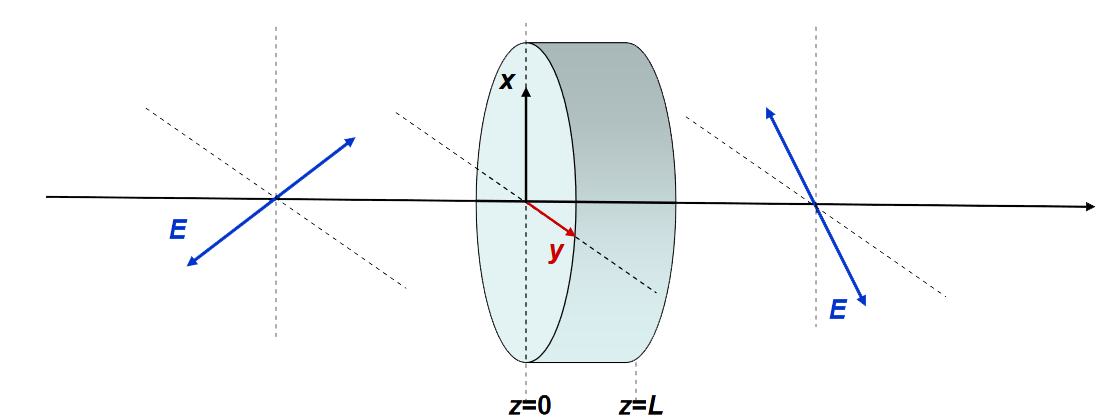
\includegraphics[width=\textwidth]{figs/HWP.PNG}
  \caption{
      A waveplate in the $xy$-plane with length $L$ with an incident
      plane wave at $z=0$ \cite{Wav_anis}. We choose $z<0$ to be region 
      1, $0<z<L$ to be region 2, and $z>L$ to be region 3. The blue lines 
      indicate the polarization of the incident field $\bv{E}_1^i$ and the
      intended polarization of the output field $\bv{E}_3$ for a HWP. The HWP
      should rotate the polarization of the input field by $\ang{90}$.
  }
  \label{fig:HWP}
\end{figure}
A HWP and QWP will be designed using the equations outlined in the theory
section of this report. Figure \ref{fig:HWP} outlines the coordinate system
and location of the waveplates that will be designed, and also shows the
intended polarization of the incident and transmitted fields for a HWP. This
diagram will be reused to design a QWP, but the designed $L$ and the intended
output polarization will be different.


% -------------------------------------------------------- Half-Waveplate Design
\subsection{Half-Waveplate Design}
By inspection, it was already shown in Equations \eqref{eq:NI_Ei}, 
\eqref{eq:NI_Et} that linearly polarized (LP) incident light in either 
purely $\bv{\hat{x}}$ or $\bv{\hat{y}}$ would stay linearly polarized inside
the anisotropic device and if the process was repeated for the second boundary
at $z=L$ it would be seen that the output field maintains the same polarization
at the input field. We will see that one possible design for a HWP uses the 
fact that the fields in the $\bv{\hat{x}}$ and $\bv{\hat{y}}$ directions travel
at different speeds in the anisotropic medium to cause a $\pi$ phase shift on
one of the axes such that the output field $\bv{E}_3$ would be polarized in 
$(-\bv{\hat{x}} + \bv{\hat{y}})/\sqrt{2}$ if the incident light $\bv{E}_{1}$ was
polarized in $(\bv{\hat{x}} + \bv{\hat{y}})/\sqrt{2}$.

We have already shown that an incident field propagating in $+z$ LP in the
$(\bv{\hat{x}} + \bv{\hat{y}})/\sqrt{2}$ direction becomes
\begin{equation}\label{eq:E2t}
  \bv{E}_2^t(z) = \frac{E_0}{\sqrt{2}}\left[\bv{\hat{x}}T_{12}^ee^{-j\beta^e z}
   + \bv{\hat{y}}T_{12}^oe^{-j\beta^o z}\right]
\end{equation}
inside the uniaxial medium. Here we will use the subscript to denote
which medium the EM wave is in, and the superscript to denote the boundaries 
that the EM wave has crossed. Now, if we want to find the case where the 
$\bv{\hat{x}}$ component of the electric field becomes $-\bv{\hat{x}}$, at 
the second boundary $z=L$, we can choose
\begin{equation}\label{eq:L_HWP}
  L(\beta^e-\beta^o) = (2m+1)\pi
  \quad\mathrm{for}\quad
  \forall m \in \mathbb{Z}
\end{equation}
where $\mathbb{Z}$ is the set of all integers \cite{Wav_anis}. 
When we rearrange Equation 
\eqref{eq:L_HWP} we obtain a relationship which we can use to rewrite
Equation \eqref{eq:E2t}
$$
  L\beta^e = (2m+1)\pi + L\beta^o
$$
So the field in the device at $z=L$ becomes
\begin{equation}\label{eq:E2t_L}
  \bv{E}_2^t(z) = \frac{E_0}{\sqrt{2}}e^{-j\beta^oL}
  \left[\bv{\hat{x}}T_{12}^ee^{-j(2m+1)\pi}
   + \bv{\hat{y}}T_{12}^o\right]
   = \frac{E_0}{\sqrt{2}}e^{-j\beta^oL}
   \left[-\bv{\hat{x}}T_{12}^e
    + \bv{\hat{y}}T_{12}^o\right]
\end{equation}
When we consider the transmission on the second boundary we obtain that the
transmitted field at the output $\bv{E}_{3}^{tt}$ becomes
\begin{equation}\label{eq:E3tt}
  \bv{E}_3^{tt}(z) = \frac{E_0}{\sqrt{2}}e^{-j\beta^oL}
  \left[-\bv{\hat{x}}T_{12}^e T_{23}^e
   + \bv{\hat{y}}T_{12}^o T_{23}^o\right]e^{-j\beta_0(z-L)}
\end{equation}
We see that our device does impart a phase shift of $\beta^oL$ on the output
field but this not a concern if we are focused on just the polarization. 
However, what is a concern is the transmission coefficients. It should be noted
that if $T^e = T^o$, then our device has no axis dependent phase retarding 
properties. This is because of the definition of the transmission coefficient
$$
T_{12} = \frac{2\eta_2}{\eta_1 + \eta_2}
$$
If we had $T^e = T^o$, it would imply $\epsilon^e=\epsilon^o$ and consequently
$\beta^e=\beta^o$. So it should be noted that a HWP of this design will not
create a perfect polarization shift of $\ang{90}$. However, if we have
\begin{equation}\label{eq:delta_T}
  \Delta T = |T_{12}^e T_{23}^e - T_{12}^o T_{23}^o| \approx 0
\end{equation}
then we have a device that does create the necessary phase retardation and gets
us very close to our desired functionality of a $\ang{90}$ polarization shift.

We have not included reflections in our discussion so far, and this was because
the base functionality of the HWP was being designed. But, we know that because
this is a two interface device, that there are an infinite number of
reflections that decrease in amplitude between the two boundaries. It should be
mentioned that we are not considering the curved boundary of the device as it 
is assumed that the incident plane wave does not fully cover the plate of the 
device.

Picking up from where we left off, if we consider the reflected light from the
boundary $z = L$, we find that the reflected field in $\bv{\hat{x}}$ is given by
\begin{equation}\label{eq:E2tr_x}
  E_{x,2}^{tr}(z) = \frac{E_0}{\sqrt{2}}e^{-j\beta^eL}
  T_{12}^e \Gamma_{23}^e e^{j\beta^e(z-L)}
\end{equation}
When we consider the reflection of this $-\bv{\hat{z}}$ propagating wave 
on the 1-2 boundary, and use the fact that if the material in region 3 is the 
same as region 1 ($\Gamma^e_{21} = \Gamma^e_{23}$), we find
\begin{equation}\label{eq:E2trr_x}
  E_{x,2}^{trr}(z) = \frac{E_0}{\sqrt{2}}e^{-j2\beta^eL}
  T_{12}^e \left(\Gamma_{23}^e\right)^2 e^{-j\beta^ez}
\end{equation}
Then, if we consider the transmission of this wave through the 2-3 boundary, we
find
\begin{equation}\label{eq:E3trrt_x}
  E_{x,3}^{trrt}(z) = \frac{E_0}{\sqrt{2}}e^{-j3\beta^eL}
  T_{12}^e \left(\Gamma_{23}^e\right)^2T_{23}^e e^{-j\beta_0 (z-L)}
\end{equation}
We could repeat this process indefinitely, but it can be seen that each trip
through the uniaxial material imparts a further phase shift on the propagating
wave, which is undesirable. But, these phase shifted reflections are decreasing
in amplitude $\Gamma^e_{23}<1$. Fortunately, we do not need to replicate this
process to evaluate the $\bv{\hat{y}}$ components of the field as we can simply
replace all extraordinary coefficients ($T^e$, $\Gamma^e$, $\beta^e$) with their
respective ordinary components and the problem is solved. Hence
\begin{equation}\label{eq:E3trrt_y}
  E_{y,3}^{trrt}(z) = \frac{E_0}{\sqrt{2}}e^{-j3\beta^oL}
  T_{12}^o \left(\Gamma_{23}^o\right)^2T_{23}^o e^{-j\beta_0 (z-L)}
\end{equation}
Looking at the relationships between Equations 
\eqref{eq:E3tt}, \eqref{eq:L_HWP}, \eqref{eq:E3trrt_x}, and \eqref{eq:E3trrt_y}
we see that, because we have a
relatively simple problem, it is possible to neatly represent the total 
output field in $\bv{\hat{x}}$ compactly as a series
\begin{equation}\label{eq:E3x_tot_HWP}
  E_{x,3}(z) = \frac{E_0}{\sqrt{2}}e^{-j(\beta_0(z-L))}\sum_{n=0}^\infty 
  T_{12}^e \left(\Gamma_{23}^e\right)^{2n}T_{23}^e
  e^{-j(2n+1)\left[\beta^oL + \pi(2m+1)\right]}
\end{equation}
And for the output field in $\bv{\hat{y}}$ we obtain
\begin{equation}\label{eq:E3y_tot_HWP}
  E_{y,3}(z) = \frac{E_0}{\sqrt{2}}e^{-j(\beta_0(z-L))}\sum_{n=0}^\infty 
  T_{12}^o \left(\Gamma_{23}^o\right)^{2n}T_{23}^o
  e^{-j(2n+1)\beta^oL}
\end{equation}
We can repeat this analysis to find a series solution for $E_{x,2}(z)$ and
$E_{y,2}(z)$ to find
\begin{equation}
  \begin{aligned}
  E_{x,2}(z) = & \frac{E_0}{\sqrt{2}}T_{12}^e\sum_{n=0}^\infty 
   \left(\Gamma_{23}^e\right)^{2n}e^{-j2n\left[\beta^oL + \pi(2m+1)\right]}
   e^{-j\beta^e z}\\ &+ 
   \left(\Gamma_{23}^e\right)^{2n+1}e^{-j(2n+1)\left[\beta^oL + \pi(2m+1)\right]}
   e^{j\beta^e (z-L)}\\
  \end{aligned}
\end{equation}
and 
\begin{equation}
  \begin{aligned}
  E_{y,2}(z) = & \frac{E_0}{\sqrt{2}}T_{12}^o\sum_{n=0}^\infty 
   \left(\Gamma_{23}^o\right)^{2n}e^{-j2n\beta^oL}
   e^{-j\beta^o z}\\ &+ 
   \left(\Gamma_{23}^o\right)^{2n+1}e^{-j(2n+1)\beta^oL}
   e^{j\beta^o (z-L)}\\
  \end{aligned}
\end{equation}

For the case of the HWP it should be noted that the round trip reflections will 
always yield $-\bv{\hat{x}}$ from the term  
$e^{-j(2n+1)\pi(2m+1)} = -1$ for any $n$, but the 
fields at $z=L$ will keep being phase shifted by the factor of 
$e^{-j(2n+1)\beta^oL}$ for each round trip ($n$ can be thought of as the number 
of round trips after first contact with the 2-3 boundary). These phase delays
will cause interference at the output, but are not a strong concern if
$(\Gamma_{23}^e)^{2n} \ll 1$ and $(\Gamma_{23}^e)^{2n} \ll 1$. We will discuss
this further when we evaluate a designed quartz HWP. Furthermore, it should be
noted that the waveplate will only cause a $\ang{90}$ polarization shift if the
incident light is polarized roughly $\pm\ang{45}$ in the $xy$ plane. This is 
satisfactory for most HWP applications. Lastly, the output $\bv{H}(z)$ field
for the HWP is given by applying the impedance in region 3 to Equations
\eqref{eq:E3x_tot_HWP}, \eqref{eq:E3y_tot_HWP} \cite{Balanis-2012}
\begin{equation}\label{eq:H3}
  \bv{H}_3(z) = \frac{1}{\eta_0}\bv{E}_3(z)
\end{equation}

% ----------------------------------------------------- Quarter-Waveplate Design
\subsection{Quarter-Waveplate Design}
Now that we have introduced the HWP design, we will now design the QWP with
the same setup (Figure \ref{fig:HWP}). To turn LP incident light into RHCP or
LHCP light we want to delay the phase of the $\bv{\hat{x}}$ field by a phase of
$\pi/2$ or $-\pi/2$. We see that we have already provided the equations
necessary to perform this task, the only difference we must make here is that
we must change Equation \eqref{eq:L_HWP} to be
\begin{equation}\label{eq:L_QWP}
  L(\beta^e-\beta^o) = (2m+1)\frac{\pi}{2}
  \quad\mathrm{for}\quad
  \forall m \in \mathbb{Z}
\end{equation}
depending on whether $m$ is odd or even we will obtain right- or left-handed
circularly polarized light. The analysis we performed to find $\bv{E}_3(z)$ is 
also still valid, but the phase shift of the light at the output will be
different. We can rewrite Equations \eqref{eq:E3x_tot_HWP} and 
\eqref{eq:E3x_tot_HWP} to be
\begin{equation}\label{eq:E3x_tot_QWP}
  E_{x,3}(z) = \frac{E_0}{\sqrt{2}}e^{-j(\beta_0(z-L))}\sum_{n=0}^\infty 
  T_{12}^e \left(\Gamma_{23}^e\right)^{2n}T_{23}^e
  e^{-j(2n+1)\left[\beta^oL + (2m+1)\pi/2\right]}
\end{equation}
and
\begin{equation}\label{eq:E3y_tot_QWP}
  E_{y,3}(z) = \frac{E_0}{\sqrt{2}}e^{-j(\beta_0(z-L))}\sum_{n=0}^\infty 
  T_{12}^o \left(\Gamma_{23}^o\right)^{2n}T_{23}^o
  e^{-j(2n+1)\beta^oL}
\end{equation}
respectively.  We will omit the reflected fields as we have already solved them
in the previous section, and we care more about how these reflected fields
degrade the output field, instead of their equations. 
Equation \eqref{eq:H3} still provides the relationship between the
$\bv{E}_3(z)$ and $\bv{H}_3(z)$ fields in medium 3. From Equation 
\eqref{eq:E3x_tot_QWP} it can be seen that for even $n$ the $\bv{\hat{x}}$
output field is shifted by a factor of $-j = e^{-j\pi/2}$ relative to the
phase of the same $n$ $\bv{\hat{y}}$ field. For odd $n$, this becomes a factor
of $j = e^{-j\pi/2}$. The means that the reflections flip between right-handed 
and left-handed. Just as before, each round trip reflection adds an additional
phase of $e^{-j2\beta^oL}$.


% ---------------------------------------------------------- Designed Waveplates
\subsection{Designed Waveplates}
Now that we have rigorously solved for the output fields $\bv{E}_3(z)$ and 
$\bv{H}_3(z)$, we are able to design a HWP and QWP using quartz. The 
parameters used for this design are shown in Table \ref{tb:param_1}. The 
computed transmission and reflection coefficients are shown in Table 
\ref{tb:param_2}.

\begin{table}[htbp]
  \centering
  \begin{tabular}{ccccccc}
    $\lambda$ (nm) & $\epsilon^e$ & $\epsilon^o$ & 
    $\beta^e$ ($\si{\micro m}^{-1}$) & $\beta^o$ ($\si{\micro m}^{-1}$)
    & $\eta^e$ ($\si{\ohm}$) & $\eta^o$ ($\si{\ohm}$)\\
    \hline\hline
    590 & 2.4130 & 2.3847 & 16.543 & 16.445 & 242.5 & 244.0\\
  \end{tabular}
  \caption{Table of parameters for waveplate design. Relative permittivity
  computed from \cite{GHOSH199995}. Parameters $\beta^e$, $\beta^o$, $\eta^e$, 
  and   $\eta^e$ were determined from the relative permittivities.}
  \label{tb:param_1}
\end{table}
\begin{table}[htbp]
  \centering
  \begin{tabular}{cccccccc}
    $\Gamma_{12}^e$ & $\Gamma_{12}^o$ & $\Gamma_{23}^e$ & $\Gamma_{23}^o$ &
    $T_{12}^e$ & $T_{12}^o$ & $T_{23}^e$ & $T_{23}^o$\\ \hline\hline
    -0.217 & -0.214 & 0.217 & 0.214 & 0.783 & 0.786 & 1.217 & 1.214\\
  \end{tabular}
  \caption{Table of computed transmission and reflection coefficients.}
  \label{tb:param_2}
\end{table}

\begin{figure}[htbp]
  \centering
  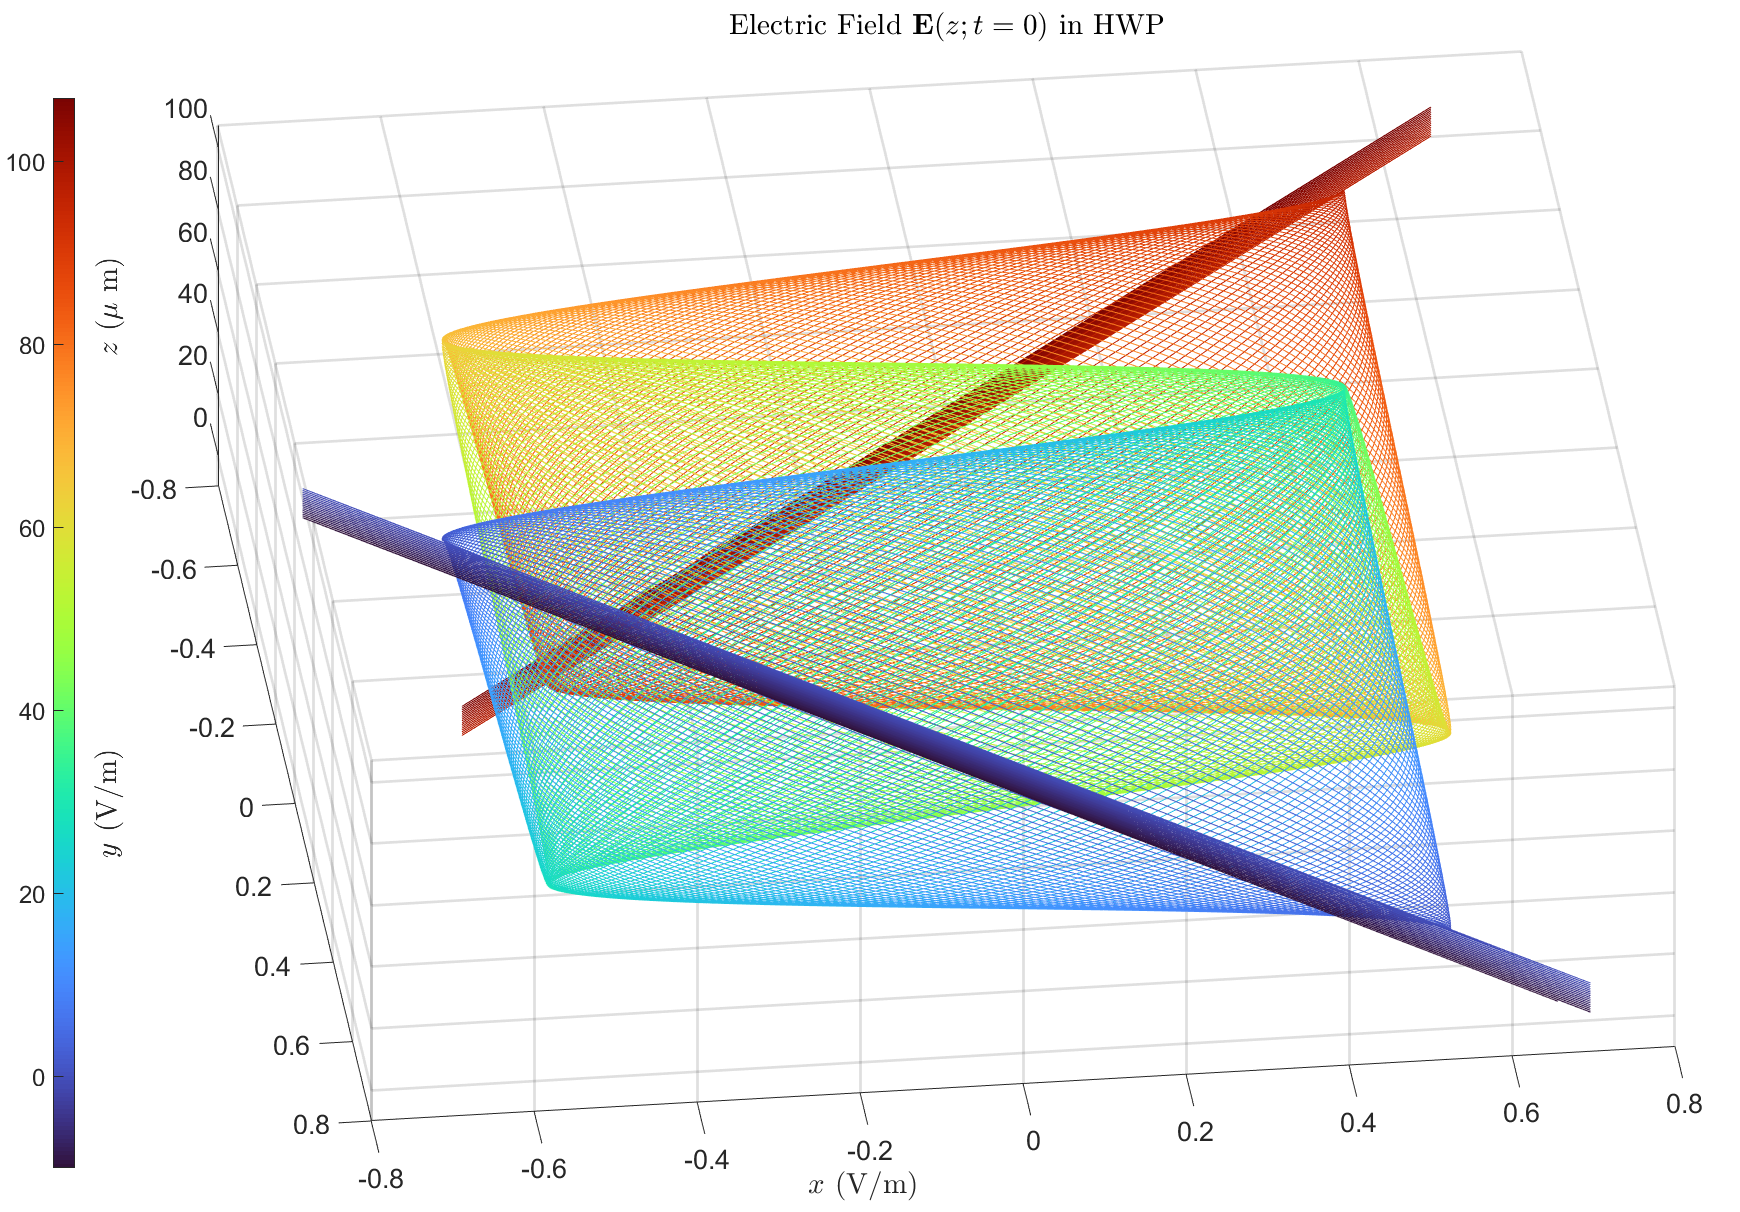
\includegraphics[width=0.9\textwidth]{figs/EfieldInHWP4.png}
  \caption{
      Forward propagating Electric Field before, inside, and after
      a quartz HWP, $L = 96.933\si{\micro \meter}$ and 
      $m=1$. Color bar helps visualize propagation in $z$.
      Reflections not considered, discontinuities of 
      $\vec{\mathscr{E}}(z; t= 0)$ would vanish they were.
  }
  \label{fig:Q_HWP}
\end{figure}

\begin{figure}[htbp]
  \centering
  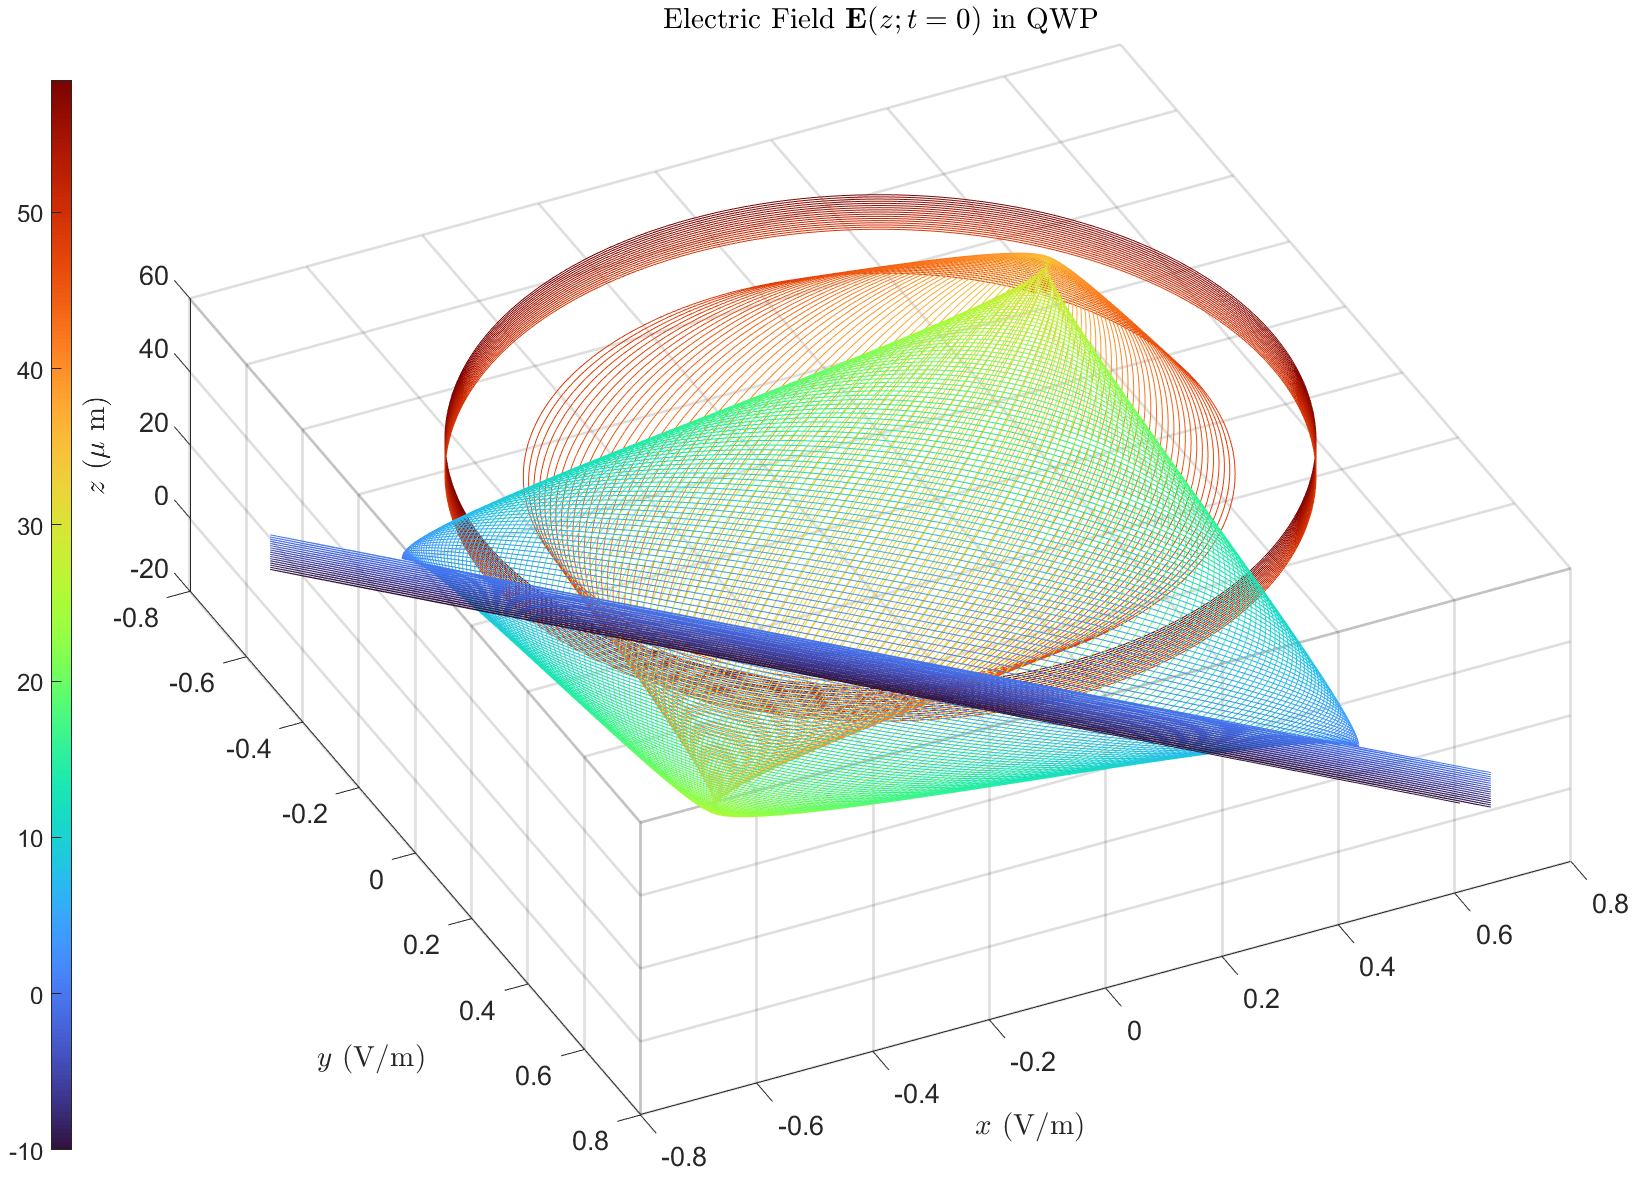
\includegraphics[width=0.9\textwidth]{figs/EfieldInQWP3.png}
  \caption{
      Forward propagating Electric Field before, inside, and after
      a quartz QWP, $L = 48.4667\si{\micro \meter}$ and 
      $m=1$. Color bar helps visualize propagation in $z$.
      Reflections not considered, discontinuities of 
      $\vec{\mathscr{E}}(z; t= 0)$ would vanish they were.
  }
  \label{fig:Q_QWP}
\end{figure}

\begin{figure}[h]
  \centering
  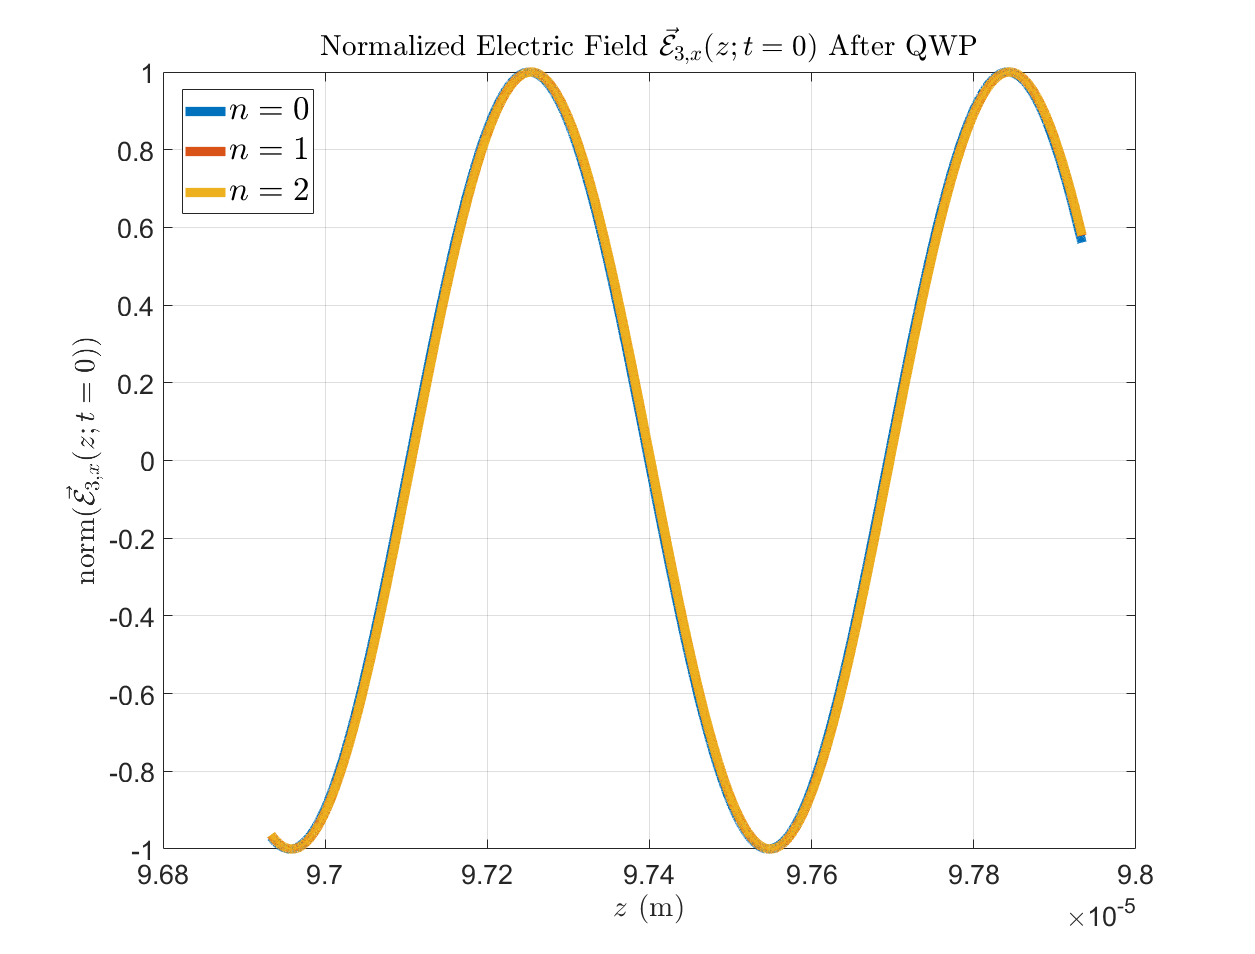
\includegraphics[width=0.8\textwidth]{figs/E3_phase.png}
  \caption{Plot of the normalized output field $\vec{\mathscr{E}}_{x,3}(z; t=0)$ for
  $z>L$ with higher order reflections considered to show the phase shift is
  minimal. $n=0$ is the 
  $\vec{\mathscr{E}}^{tt}_{x,3}(z; t=0)$ field, $n=1$ is the field given by
  $\vec{\mathscr{E}}^{tt}_{x,3}(z; t=0) + 
  \vec{\mathscr{E}}^{trrt}_{x,3}(z; t=0)$ and so on.
  }
  \label{fig:E3x_phase}
\end{figure}

To evaluate the performance of the designed devices we introduce the ratio of
the $n=1$ ($\bv{E}_3^{trrt}$) reflected power to the $n=0$ ($\bv{E}_3^{tt}$)
power 
\begin{equation}\label{eq:RP}
R^\% = \frac{|\bv{E}_3^{trrt}|^2}{|\bv{E}_3^{tt}|^2} \cdot 100 = 
\frac{
\left[T^e_{12}(\Gamma^e_{23})^2T^e_{23}\right]^2 + 
\left[T^o_{12}(\Gamma^o_{23})^2T^o_{23}\right]^2
}{\left[T^e_{12}T^e_{23}\right]^2 + 
\left[T^o_{12}T^o_{23}\right]^2} \cdot 100
\end{equation}
The value of $R^\%$ will give us a sense of how well performing our designed
device is. If $R^\%$ is low, further reflections will be even lower and can be
neglected. The $\bv{E}_3^{trrt}$ field will cause the greatest degradation
in performance.

\begin{table}[h]
  \centering
  \begin{tabular}{ccccc}
    Plate Type & $L$ ($\si{\micro m}$) & $m$ & $\Delta T$ & $R^\%$\\\hline \hline
    HWP & 96.933 & 1 & 0.001 & 0.215\%\\\hline
    HWP & 226.178 & 3 & 0.001 & 0.215\%\\\hline
    QWP & 48.467 & 1 & 0.001 & 0.215\%\\\hline
    QWP & 113.089 & 3 & 0.001 & 0.215\%\\\hline
  \end{tabular}
  \caption{Designed quantities and performance characterization quantities}
  \label{tb:Vals}
\end{table}

Table \ref{tb:Vals} shows the determined values of $L$ for $m=1$ and $m=3$ as 
well as the discussed performance evaluating parameters. Again, $m$ could be
any integer, so these are only highlighting some of many possible lengths for
the waveplates to be. It can be seen that changing the length of the device 
has no impact on $\Delta T$ nor $R^\%$.

Figures \ref{fig:Q_HWP} and \ref{fig:Q_QWP} show the fields 
$\vec{\mathscr{E}}_1^i(z; t = 0)$, $\vec{\mathscr{E}}_2^{t}(z; t = 0)$, and 
$\vec{\mathscr{E}}_3^{tt}(z; t = 0)$ for both the HWP and QWP respectively.
The discontinuities at $z=0$ and $z=L$ arise from the fact that the reflected
fields are not considered. The BC require that the tangential components
of the all fields be continuous at the boundary, without considering the 
reflected waves our plot simply would not show this. Figure \ref{fig:E3x_phase}
shows the output field $\vec{\mathscr{E}}_{x,3}(z; t=0)$ with higher order
reflections considered. It can be seen that reflections beyond 
$\vec{\mathscr{E}}^{trrt}_{x,3}(z; t=0)$ do not have much impact on the 
phase of the output field.



% ------------------------------------------------------------------------------
% Discussion
% ------------------------------------------------------------------------------
\section{Discussion}
Now that we have designed a HWP and QWP for normally incident light, provided
some crude metrics to evaluate its performance, and plotted the fields inside of
the waveplates, we will further discuss their performance and utility.

% ------------------------------------------------------------ Oblique Incidence
\subsection{Oblique Incidence}
\begin{figure}[htbp]
  \centering
  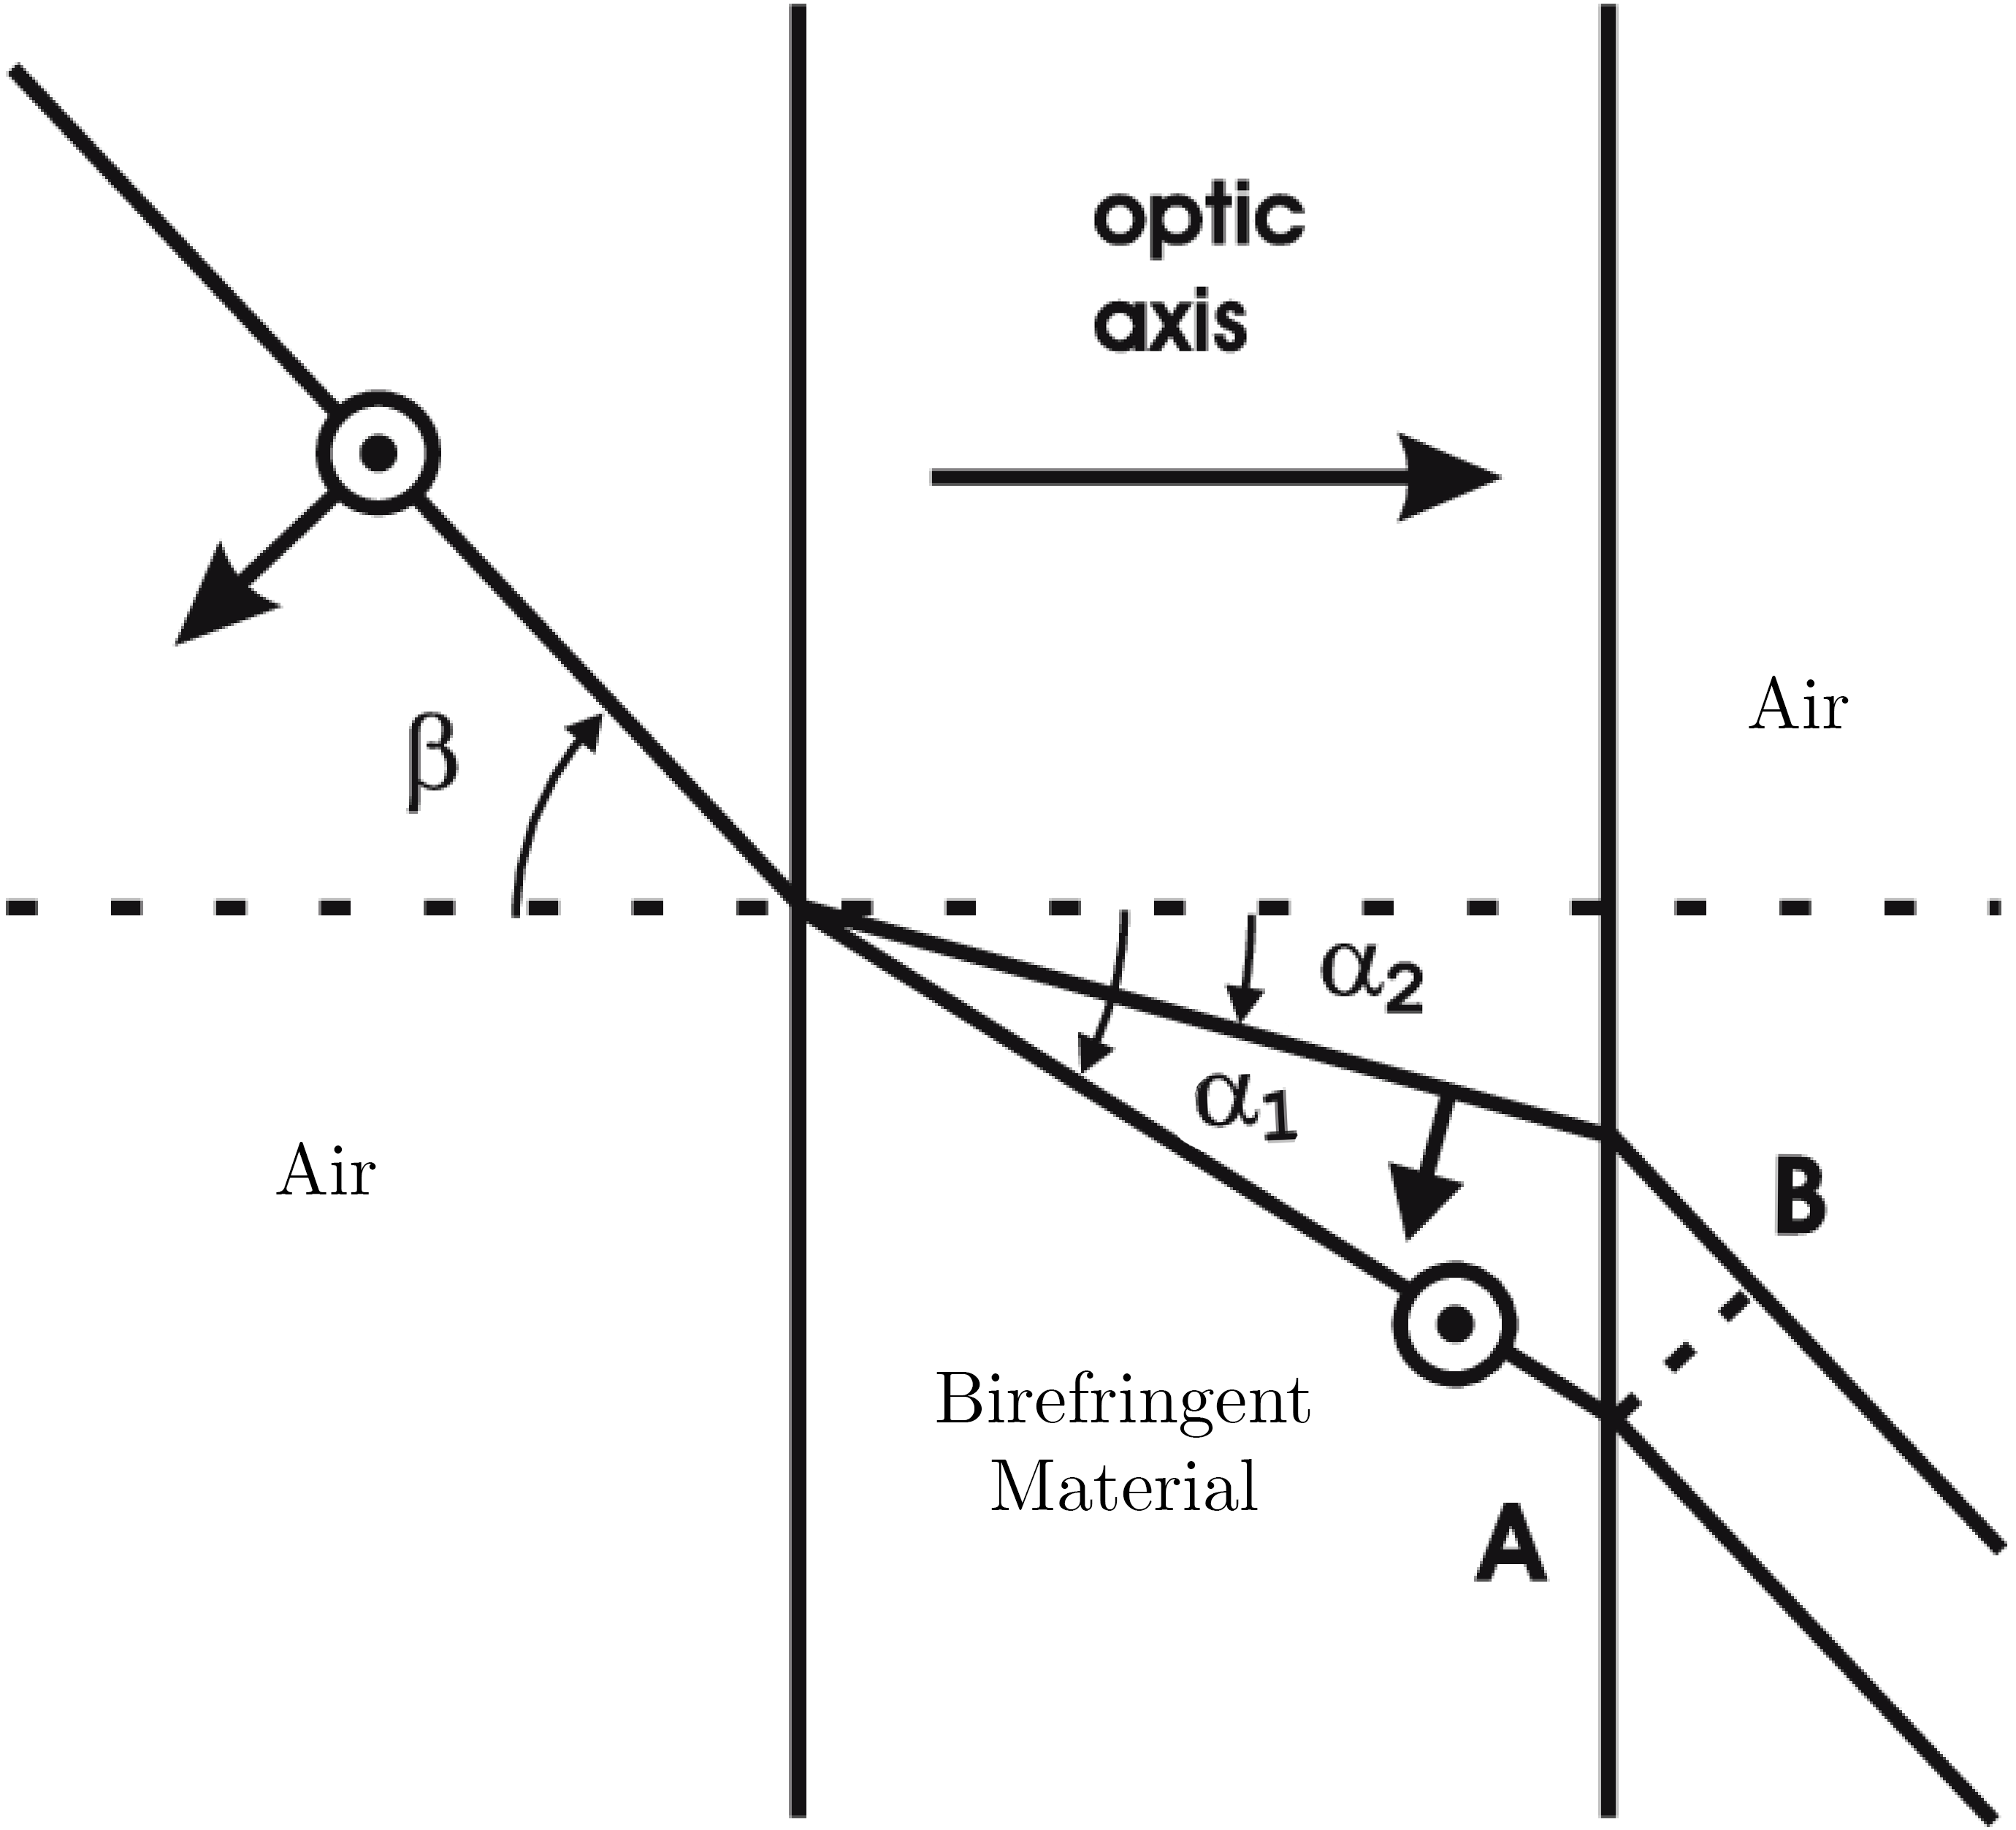
\includegraphics[width=0.5\textwidth]{figs/Birefringence.png}
  \caption{
      We obtain two spatially separated propagating fields when 
      we consider
      the case of oblique incidence on a birefringent 
      material \cite{BR_IM}.
  }
  \label{fig:BR}
\end{figure}
\begin{figure}[h]
  \centering
  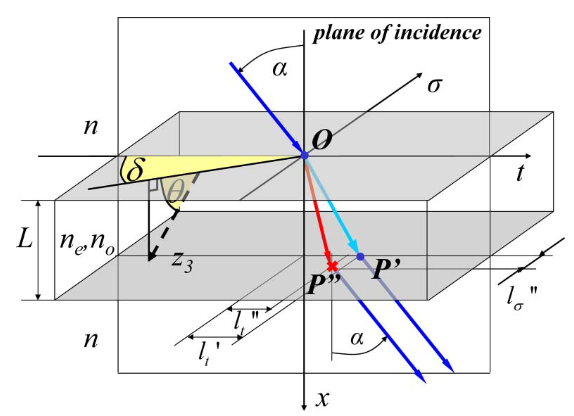
\includegraphics[width=0.7\textwidth]{figs/WP_OI_setup.PNG}
  \caption{ ``Ordinary and extraordinary transmission
  through a uniaxial plane-parallel plate immersed in an isotropic
  medium. $\theta$ is the angle between the optical axis and the interface. 
  $\delta$ is the angle between the plane of incidence and the optical axis 
  projection on the interface.'' $\alpha$ is the angle of incidence.
  \cite{OBI_phase}. }
  \label{fig:obi_set}
\end{figure}

Our analysis to this point has focused on the case of normal incidence, but
what if we desire our device to perform in the case of oblique incidence?
Well, unforunately, a waveplate of this design is not able to have its 
intended effects for the case of oblique incidence. We saw earlier that 
we needed to employ two different transmission and reflection coefficients
for the fields in $\bv{\hat{x}}$ and $\bv{\hat{y}}$. In our example, the 
extraordinary and ordinary coefficients respectively. So to consider oblique
incidence, we must also apply Snell's law twice as well, shown in Equations 
\eqref{eq:snell_theta_e} and \eqref{eq:snell_theta_o}.
\begin{equation}\label{eq:snell_theta_e}
  \theta^e_t = \sin^{-1}\left(\frac{\beta_0}{\beta^e}\sin(\theta_i)\right)
\end{equation}
\begin{equation}\label{eq:snell_theta_o}
  \theta^o_t = \sin^{-1}\left(\frac{\beta_0}{\beta^o}\sin(\theta_i)\right)
\end{equation}
We know that $\beta^e$ and $\beta^o$ are often similar for many materials, but
still differ. As such, it can be seen that for cases of very shallow incidence,
$\theta_i \approx \ang{0}$
that $\sin(\theta_i) \approx 0$ which means that despite the small difference
between $\beta^e$ and $\beta^o$ the waveplate will still function mostly as
intended. In the case of the QWP the slightly eliptically polarized output
field would become even more eliptically polarized as the slightly different
angles of refraction would cause a slight additional phase shift on one of the
fields. But, for the case where $\sin{\theta_i}$ is not approximately zero,
we see that Equations \eqref{eq:snell_theta_e} and \eqref{eq:snell_theta_o}
yield very different angles of transmission. Figure \ref{fig:BR} shows what
the transmitted fields would look like. We see that the transmitted fields
become more spatially separated as they propagate through the anisotropic
material, and that they are spatially separated at the output.
We call this effect, when we have two 
refracted EM waves that originate from one incident ray, birefringence. 
Furthermore, we call the materials that this effect happens in 
\textit{birefringent materials}. Anisotropic materials usually exhibit this 
property because their permittivities are directionally dependent.

\begin{figure}[htp]
  \centering
  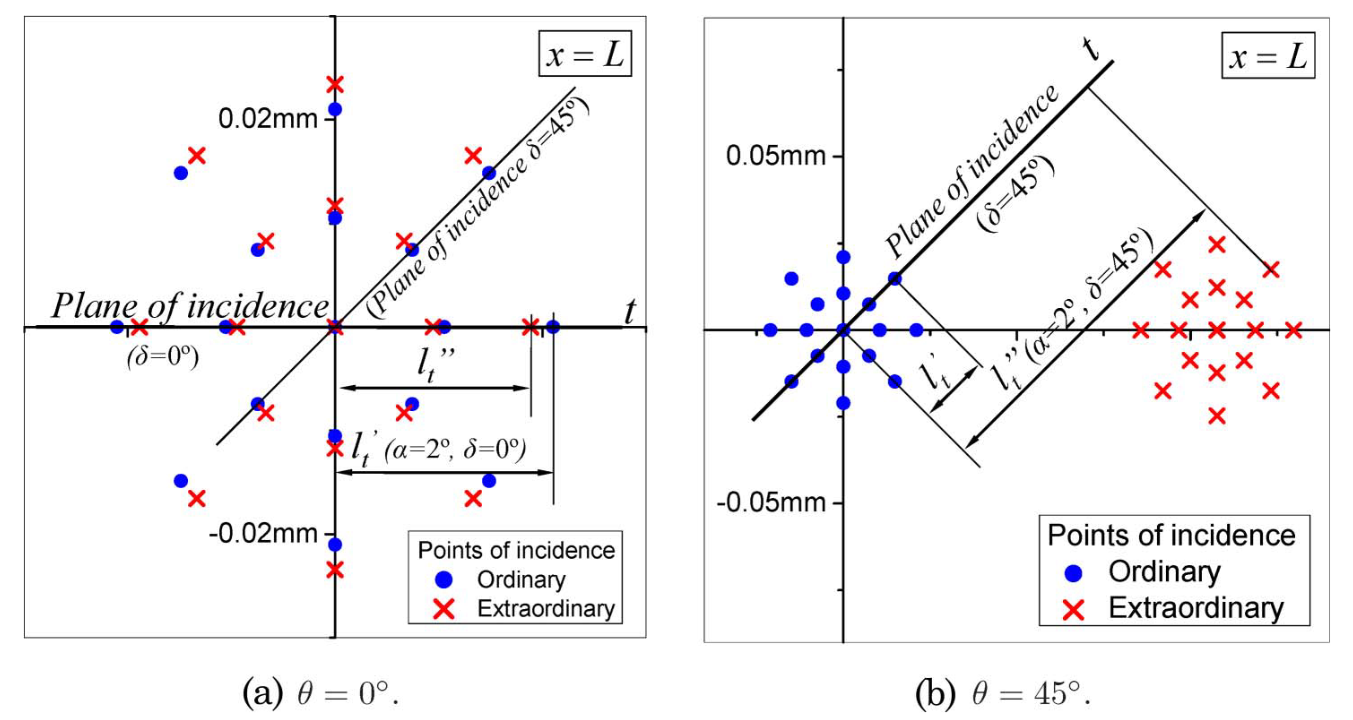
\includegraphics[width=0.8\textwidth]{figs/WP_OI.PNG}
  \caption{Spatial separation of the ordinary and extraordinary rays at the 
  output plane of a calcite plate where 
  the  angle of incidence normal to the surface is given by $\alpha$ and the 
  azimuthal angle $\delta$ relative to the optical axis of the device, shown 
  in Figure \ref{fig:obi_set} (a) the case where the materials crystalline
  structure is oriented with an ordinary and extraordinary axis parallel to the
  surface $\theta=\ang{0}$
  and (b) the case of the crystalline structure being aligned with 
  $\theta=\ang{45}$ \cite{OBI_phase}.}
  \label{fig:obi}
\end{figure}

\begin{figure}[htp]
  \centering
  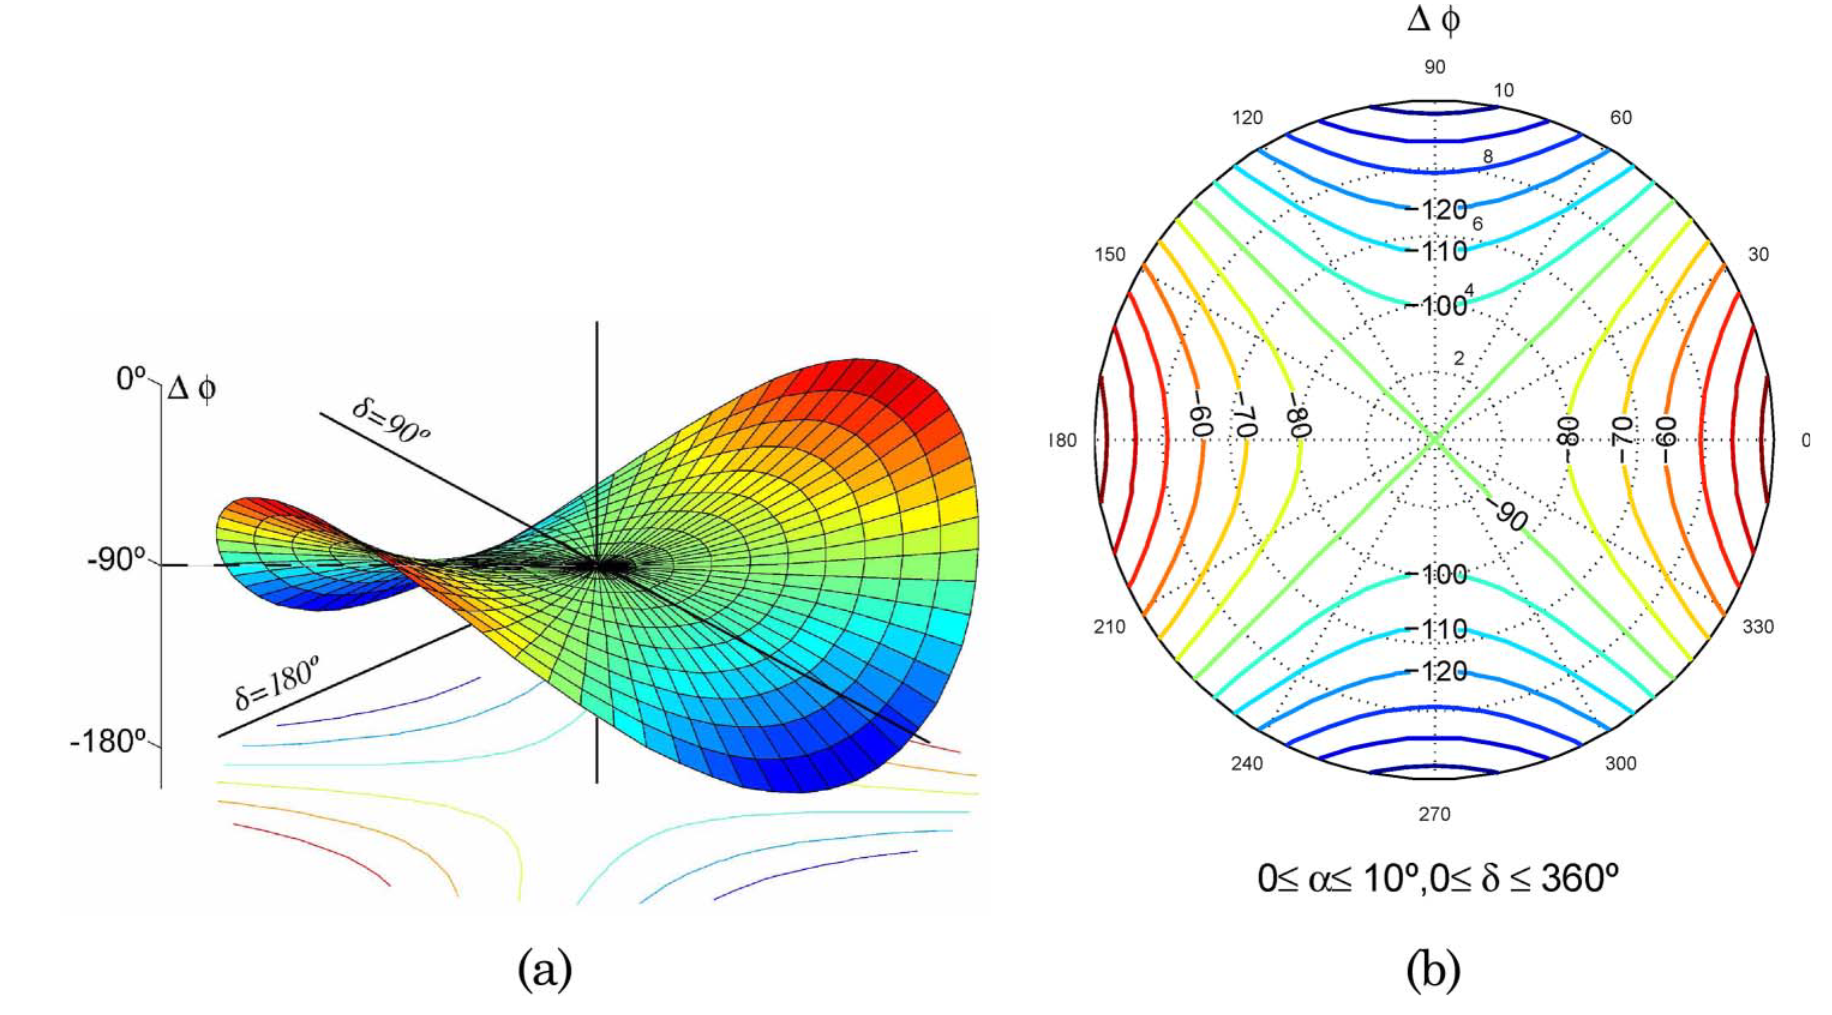
\includegraphics[width=0.9\textwidth]{figs/PhaseDelay.PNG}
  \caption{Oblique incidence phase delay $\Delta \phi (\alpha,\delta)$ 
  at the output plane of a quartz half-waveplate
  where the
  angle of incidence normal to the surface is given by $\alpha$ and the 
  azimuthal angle $\delta$ relative to the optical axis of the device as shown 
  in Figure \ref{fig:obi_set}. On the plots, the azimuthal angle of the
  coordinate system corresponds to the various angles of $\delta$ and the radial
  direction on the graphs indicates $\ang{0} < \alpha < \ang{10}$
   \cite{OBI_phase}.}
  \label{fig:obi_phase}
\end{figure}

It should
be noted that in our example, if we had an obliquely incident field, where
its $\bv{E}$ field was present in both $\bv{\hat{x}}$ and $\bv{\hat{z}}$, that
there would only be one transmitted wave. While we already noted that a field
purely in $\bv{\hat{y}}$ would not have its polarization changed by the
waveplate, if it was obliquely incident, it would also not create multiple
waves inside of the uniaxial material because the permittivities in the 
$\bv{\hat{y}}$ and $\bv{\hat{z}}$ are the same.



Understanding how waveplates function with oblique incidence is of particular
interest to researchers and engineers. There are many applications where
polarization transformations are desired, but ensuring normal incidence may
not be possible.



Figure \ref{fig:obi_set} shows the variables for plane wave incidence on a 
birefringent material as described in 
\textit{Phase shift formulas in uniaxial media} which will be used in 
to discuss Figure \ref{fig:obi} \cite{OBI_phase}. 
Part (a) in Figure \ref{fig:obi} shows that for 
slight obliquely incident light $\alpha =\ang{2}$ with the material having its
optical axis being normal to its surface (the designed case that we did in this
report) we see that for different orientations of this obliquely incident
light (described by $\delta$) the ordinary and extraordinary rays do not align 
at the
output plane of the device. Furthermore, if we change the optical axis of the
device, which would correspond to misalignment of the permittivity tensor,
we see that the device performance completely breaks down: 
Figure \ref{fig:obi}-b. As expected, the birefringent properties of the 
anisotropic material cause the fields to spatially diverge substantially. 
This paper supports the need to make the design 
choices articulated in the design portion of this report. Furthermore, 
the phase delay for a desired quarter-wave plate $\Delta \phi (\alpha,\delta)$ 
is shown in Figure \ref{fig:obi_phase}. For incident angles of $\alpha>\ang{4}$
we start to notice more pronounced differences between the desired phase
shift of $\ang{90}$ and the actual phase $\Delta \phi (\alpha,\delta)$ 
\cite{OBI_phase}.


% ----------------------------------------------------- Anti-Reflective Coatings
\subsection{Anti-Reflective Coatings}
Figure \ref{fig:E3x_phase} and our metric $R^\%$ showed that our designed 
waveplates work fairly well even with the internal reflections of the device.
However, to make the output field even more consistent with the desired 
polarization, anti-reflective coatings could be employed to further diminish 
the slight phase delay that the round trip reflections cause. These coatings 
could be placed on both sides of the waveplate to further couple the output
field and reduce the reflection coefficients even further. However, with the
addition of more interfaces to our device, there are more opportunities for
internal reflections, and it becomes impossible to make a neat series solution
for the problem. In our design section, we exploited the fact that we can 
describe each round trip through our device by a phase factor to get our 
analytical solution, but this becomes too tedious to perform. Such devices 
would have to be modeled with finite difference time domain method (FDTD) or 
rigorous coupled wave analysis (RCWA) \cite{FTDT,SLM_RCWA}. Both of these 
methods are numerical methods to approximate the solutions to Maxwell's 
equations and while computationally expensive, they are able to solve problems
with complex boundary conditions such as a graded index fiber or complex 
anisotropic materials such as liquid crystals.

% -------------------------------------------------------- Wavelength Dependence
\subsection{Wavelength Dependence}
The design for the QWP and HWP presented in this report neglected to consider
the case for an achromatic incident field. For Quartz, an most anisotropic
materials, their relative permittivities $\epsilon^e$ and $\epsilon^o$ are 
frequency dependent. As such, as the frequency changes the values of
$\beta^e$ and $\beta^o$ vary---meaning that the neat phase delay factors we 
related to the length will not work for the whole range of incident frequencies.
But if we can live with slight elliptically polarized light in our application,
and we choose materials such that $\beta^e$ and $\beta^o$ remain relatively
unchanged, it is possible to design a device that closely meets the desired 
performance.

However, we as engineers have more tools at our disposal, it is possible to 
couple multiple anisotropic materials together to help reduce this chromatic
dispersion. ``The most common type is crystalline quartz and magnesium fluoride 
birefringent crystals in an air-spaced design'' \cite{newport}. By making more
complicated designs, we make tradeoffs in our design criteria to make 
electromagnetic devices that meet the desired operating criteria.

% -------------------------------------------------------------- Liquid Crystals
\subsection{Liquid Crystals}
Liquid crystals are a very different type of anisotropic material that are 
highly useful for research and consumer applications. Most notable, they 
are ubiquitous in computer displays. In the display the liquid crystal is used
to modulate the polarization of a pixel's back-light such that when the 
modulated light hits the polarizing film of the display, the brightness of the
display's pixels can be independently controlled by modulated the voltage bias
on the crystal. A similar technique is used by spatial light modulators (SLM) 
which are devices that use a pixelated liquid crystal to impart a phase
delays on an incident wavefront. In both of these devices, it is the anisotropic
properties of the liquid crystal that allows for the light to be modulated.
When we apply a bias voltage we are able to change the crystalline structure
and therefore alter the optical axis of the material. Information regarding
the refractive indices $n$ and therefore the relative permittivities 
$\epsilon_r$ (in the case of non-magnetic liquid crystals) is well documented 
by Jun Li in his PHD thesis \cite{LC}. The author had initially wanted to model
liquid crystal based devices, but with no background in anisotropy this proved
to be difficult. Hence, our discussion almost 
entirely focused on uniaxial media, but this section on liquid crystals was
included for some additional background on anisotropic materials.


% ------------------------------------------------------------------------------
% Conclusion
% ------------------------------------------------------------------------------
\section{Conclusion}
This paper has provided a discussion on electromagnetic 
fields in uniaxial media, with a focus on designing waveplates for changing the 
polarization of an incident electromagnetic wave. The theoretical background was
presented, and analytical solutions were derived for half-waveplate and 
quarter-waveplate designs using a quartz crystal for 590 nm normally incident 
light. The performance of the designed waveplates was evaluated, and the 
challenges associated with waveplate design were discussed. This paper serves 
as an introduction into anisotropic electromagnetic device design.


%%%%%%%%%%%%%%%%%%%%%%% Backmatter %%%%%%%%%%%%%%%%%%%%%%%%%

\begin{backmatter}
  \bmsection{Funding}
  This research is unfunded.

  \bmsection{Acknowledgments}
  The author thanks T. Saule
  for his contributions to the author's understanding.

  \bmsection{Disclosures}
  The authors declare no conflicts of interest.

  \bmsection{Data availability}  \LaTeX and MATLAB code for this project and
  its reports can be found on the author's github and are accessible 
  at the following link:
  \url{https://github.com/kevinlindstrom/ECE5201}
\end{backmatter}

%%%%%%%%%%%%%%%%%%%%%%% References %%%%%%%%%%%%%%%%%%%%%%%%%

% Use Bibtex
\bibliography{ECE5201_Citations}


\end{document}
